% Created by tikzDevice version 0.10.1 on 2017-10-05 07:17:47
% !TEX encoding = UTF-8 Unicode
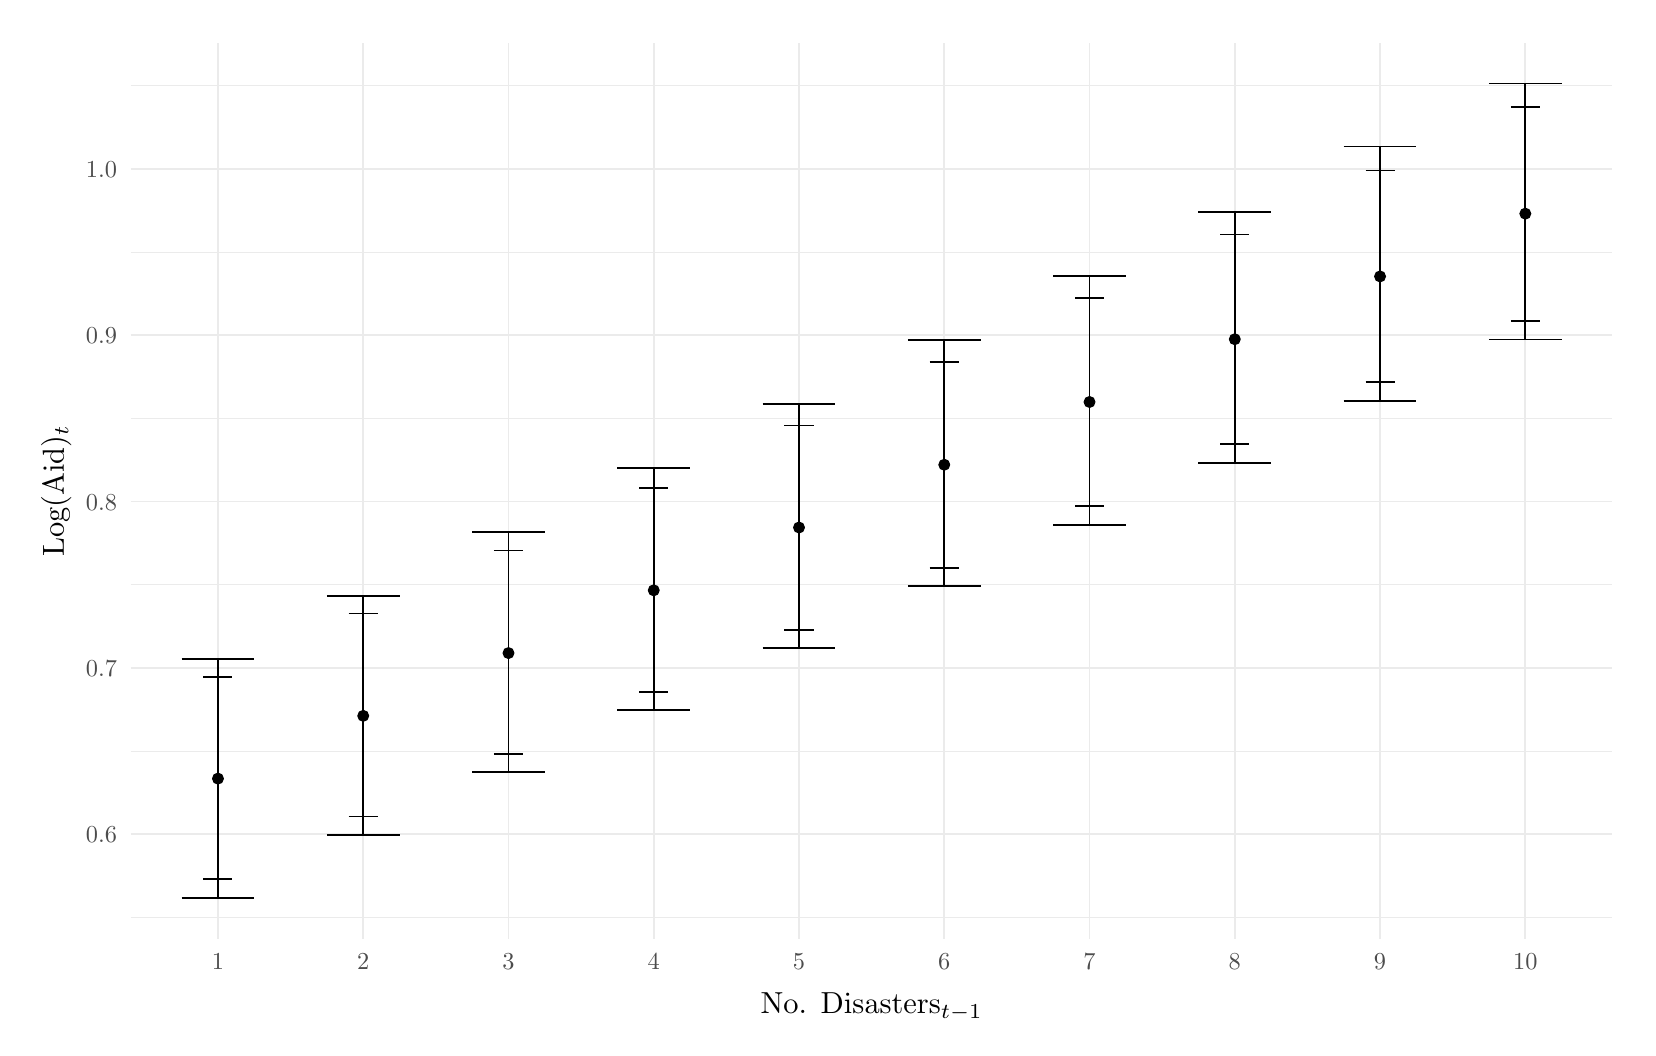
\begin{tikzpicture}[x=1pt,y=1pt]
\definecolor{fillColor}{RGB}{255,255,255}
\path[use as bounding box,fill=fillColor,fill opacity=0.00] (0,0) rectangle (578.16,361.35);
\begin{scope}
\path[clip] (  0.00,  0.00) rectangle (578.16,361.35);
\definecolor{drawColor}{RGB}{255,255,255}
\definecolor{fillColor}{RGB}{255,255,255}

\path[draw=drawColor,line width= 0.6pt,line join=round,line cap=round,fill=fillColor] (  0.00,  0.00) rectangle (578.16,361.35);
\end{scope}
\begin{scope}
\path[clip] ( 37.27, 32.09) rectangle (572.66,355.85);
\definecolor{fillColor}{RGB}{255,255,255}

\path[fill=fillColor] ( 37.27, 32.09) rectangle (572.66,355.85);
\definecolor{drawColor}{gray}{0.92}

\path[draw=drawColor,line width= 0.3pt,line join=round] ( 37.27, 39.85) --
	(572.66, 39.85);

\path[draw=drawColor,line width= 0.3pt,line join=round] ( 37.27, 99.95) --
	(572.66, 99.95);

\path[draw=drawColor,line width= 0.3pt,line join=round] ( 37.27,160.04) --
	(572.66,160.04);

\path[draw=drawColor,line width= 0.3pt,line join=round] ( 37.27,220.13) --
	(572.66,220.13);

\path[draw=drawColor,line width= 0.3pt,line join=round] ( 37.27,280.23) --
	(572.66,280.23);

\path[draw=drawColor,line width= 0.3pt,line join=round] ( 37.27,340.32) --
	(572.66,340.32);

\path[draw=drawColor,line width= 0.6pt,line join=round] ( 37.27, 69.90) --
	(572.66, 69.90);

\path[draw=drawColor,line width= 0.6pt,line join=round] ( 37.27,129.99) --
	(572.66,129.99);

\path[draw=drawColor,line width= 0.6pt,line join=round] ( 37.27,190.09) --
	(572.66,190.09);

\path[draw=drawColor,line width= 0.6pt,line join=round] ( 37.27,250.18) --
	(572.66,250.18);

\path[draw=drawColor,line width= 0.6pt,line join=round] ( 37.27,310.28) --
	(572.66,310.28);

\path[draw=drawColor,line width= 0.6pt,line join=round] ( 68.76, 32.09) --
	( 68.76,355.85);

\path[draw=drawColor,line width= 0.6pt,line join=round] (121.25, 32.09) --
	(121.25,355.85);

\path[draw=drawColor,line width= 0.6pt,line join=round] (173.74, 32.09) --
	(173.74,355.85);

\path[draw=drawColor,line width= 0.6pt,line join=round] (226.23, 32.09) --
	(226.23,355.85);

\path[draw=drawColor,line width= 0.6pt,line join=round] (278.72, 32.09) --
	(278.72,355.85);

\path[draw=drawColor,line width= 0.6pt,line join=round] (331.21, 32.09) --
	(331.21,355.85);

\path[draw=drawColor,line width= 0.6pt,line join=round] (383.70, 32.09) --
	(383.70,355.85);

\path[draw=drawColor,line width= 0.6pt,line join=round] (436.19, 32.09) --
	(436.19,355.85);

\path[draw=drawColor,line width= 0.6pt,line join=round] (488.68, 32.09) --
	(488.68,355.85);

\path[draw=drawColor,line width= 0.6pt,line join=round] (541.17, 32.09) --
	(541.17,355.85);
\definecolor{drawColor}{RGB}{0,0,0}

\path[draw=drawColor,line width= 0.6pt,line join=round] ( 63.51,126.75) --
	( 74.01,126.75);

\path[draw=drawColor,line width= 0.6pt,line join=round] ( 68.76,126.75) --
	( 68.76, 53.70);

\path[draw=drawColor,line width= 0.6pt,line join=round] ( 63.51, 53.70) --
	( 74.01, 53.70);

\path[draw=drawColor,line width= 0.6pt,line join=round] (116.00,149.61) --
	(126.50,149.61);

\path[draw=drawColor,line width= 0.6pt,line join=round] (121.25,149.61) --
	(121.25, 76.34);

\path[draw=drawColor,line width= 0.6pt,line join=round] (116.00, 76.34) --
	(126.50, 76.34);

\path[draw=drawColor,line width= 0.6pt,line join=round] (168.49,172.38) --
	(178.99,172.38);

\path[draw=drawColor,line width= 0.6pt,line join=round] (173.74,172.38) --
	(173.74, 98.82);

\path[draw=drawColor,line width= 0.6pt,line join=round] (168.49, 98.82) --
	(178.99, 98.82);

\path[draw=drawColor,line width= 0.6pt,line join=round] (220.98,194.94) --
	(231.48,194.94);

\path[draw=drawColor,line width= 0.6pt,line join=round] (226.23,194.94) --
	(226.23,121.22);

\path[draw=drawColor,line width= 0.6pt,line join=round] (220.98,121.22) --
	(231.48,121.22);

\path[draw=drawColor,line width= 0.6pt,line join=round] (273.47,217.64) --
	(283.97,217.64);

\path[draw=drawColor,line width= 0.6pt,line join=round] (278.72,217.64) --
	(278.72,143.70);

\path[draw=drawColor,line width= 0.6pt,line join=round] (273.47,143.70) --
	(283.97,143.70);

\path[draw=drawColor,line width= 0.6pt,line join=round] (325.96,240.64) --
	(336.46,240.64);

\path[draw=drawColor,line width= 0.6pt,line join=round] (331.21,240.64) --
	(331.21,166.21);

\path[draw=drawColor,line width= 0.6pt,line join=round] (325.96,166.21) --
	(336.46,166.21);

\path[draw=drawColor,line width= 0.6pt,line join=round] (378.45,263.60) --
	(388.95,263.60);

\path[draw=drawColor,line width= 0.6pt,line join=round] (383.70,263.60) --
	(383.70,188.62);

\path[draw=drawColor,line width= 0.6pt,line join=round] (378.45,188.62) --
	(388.95,188.62);

\path[draw=drawColor,line width= 0.6pt,line join=round] (430.94,286.58) --
	(441.44,286.58);

\path[draw=drawColor,line width= 0.6pt,line join=round] (436.19,286.58) --
	(436.19,211.01);

\path[draw=drawColor,line width= 0.6pt,line join=round] (430.94,211.01) --
	(441.44,211.01);

\path[draw=drawColor,line width= 0.6pt,line join=round] (483.43,309.75) --
	(493.93,309.75);

\path[draw=drawColor,line width= 0.6pt,line join=round] (488.68,309.75) --
	(488.68,233.32);

\path[draw=drawColor,line width= 0.6pt,line join=round] (483.43,233.32) --
	(493.93,233.32);

\path[draw=drawColor,line width= 0.6pt,line join=round] (535.92,332.76) --
	(546.42,332.76);

\path[draw=drawColor,line width= 0.6pt,line join=round] (541.17,332.76) --
	(541.17,255.30);

\path[draw=drawColor,line width= 0.6pt,line join=round] (535.92,255.30) --
	(546.42,255.30);

\path[draw=drawColor,line width= 0.6pt,line join=round] ( 55.64,133.21) --
	( 81.88,133.21);

\path[draw=drawColor,line width= 0.6pt,line join=round] ( 68.76,133.21) --
	( 68.76, 46.80);

\path[draw=drawColor,line width= 0.6pt,line join=round] ( 55.64, 46.80) --
	( 81.88, 46.80);

\path[draw=drawColor,line width= 0.6pt,line join=round] (108.13,156.05) --
	(134.37,156.05);

\path[draw=drawColor,line width= 0.6pt,line join=round] (121.25,156.05) --
	(121.25, 69.52);

\path[draw=drawColor,line width= 0.6pt,line join=round] (108.13, 69.52) --
	(134.37, 69.52);

\path[draw=drawColor,line width= 0.6pt,line join=round] (160.62,179.16) --
	(186.86,179.16);

\path[draw=drawColor,line width= 0.6pt,line join=round] (173.74,179.16) --
	(173.74, 92.30);

\path[draw=drawColor,line width= 0.6pt,line join=round] (160.62, 92.30) --
	(186.86, 92.30);

\path[draw=drawColor,line width= 0.6pt,line join=round] (213.11,202.25) --
	(239.35,202.25);

\path[draw=drawColor,line width= 0.6pt,line join=round] (226.23,202.25) --
	(226.23,114.82);

\path[draw=drawColor,line width= 0.6pt,line join=round] (213.11,114.82) --
	(239.35,114.82);

\path[draw=drawColor,line width= 0.6pt,line join=round] (265.60,225.29) --
	(291.84,225.29);

\path[draw=drawColor,line width= 0.6pt,line join=round] (278.72,225.29) --
	(278.72,137.13);

\path[draw=drawColor,line width= 0.6pt,line join=round] (265.60,137.13) --
	(291.84,137.13);

\path[draw=drawColor,line width= 0.6pt,line join=round] (318.09,248.40) --
	(344.33,248.40);

\path[draw=drawColor,line width= 0.6pt,line join=round] (331.21,248.40) --
	(331.21,159.60);

\path[draw=drawColor,line width= 0.6pt,line join=round] (318.09,159.60) --
	(344.33,159.60);

\path[draw=drawColor,line width= 0.6pt,line join=round] (370.58,271.54) --
	(396.82,271.54);

\path[draw=drawColor,line width= 0.6pt,line join=round] (383.70,271.54) --
	(383.70,181.70);

\path[draw=drawColor,line width= 0.6pt,line join=round] (370.58,181.70) --
	(396.82,181.70);

\path[draw=drawColor,line width= 0.6pt,line join=round] (423.06,294.81) --
	(449.31,294.81);

\path[draw=drawColor,line width= 0.6pt,line join=round] (436.19,294.81) --
	(436.19,203.97);

\path[draw=drawColor,line width= 0.6pt,line join=round] (423.06,203.97) --
	(449.31,203.97);

\path[draw=drawColor,line width= 0.6pt,line join=round] (475.55,318.36) --
	(501.80,318.36);

\path[draw=drawColor,line width= 0.6pt,line join=round] (488.68,318.36) --
	(488.68,226.49);

\path[draw=drawColor,line width= 0.6pt,line join=round] (475.55,226.49) --
	(501.80,226.49);

\path[draw=drawColor,line width= 0.6pt,line join=round] (528.04,341.13) --
	(554.29,341.13);

\path[draw=drawColor,line width= 0.6pt,line join=round] (541.17,341.13) --
	(541.17,248.64);

\path[draw=drawColor,line width= 0.6pt,line join=round] (528.04,248.64) --
	(554.29,248.64);
\definecolor{fillColor}{RGB}{0,0,0}

\path[draw=drawColor,line width= 0.4pt,line join=round,line cap=round,fill=fillColor] ( 68.76, 90.00) circle (  1.96);

\path[draw=drawColor,line width= 0.4pt,line join=round,line cap=round,fill=fillColor] (121.25,112.68) circle (  1.96);

\path[draw=drawColor,line width= 0.4pt,line join=round,line cap=round,fill=fillColor] (173.74,135.36) circle (  1.96);

\path[draw=drawColor,line width= 0.4pt,line join=round,line cap=round,fill=fillColor] (226.23,158.04) circle (  1.96);

\path[draw=drawColor,line width= 0.4pt,line join=round,line cap=round,fill=fillColor] (278.72,180.73) circle (  1.96);

\path[draw=drawColor,line width= 0.4pt,line join=round,line cap=round,fill=fillColor] (331.21,203.41) circle (  1.96);

\path[draw=drawColor,line width= 0.4pt,line join=round,line cap=round,fill=fillColor] (383.70,226.09) circle (  1.96);

\path[draw=drawColor,line width= 0.4pt,line join=round,line cap=round,fill=fillColor] (436.19,248.77) circle (  1.96);

\path[draw=drawColor,line width= 0.4pt,line join=round,line cap=round,fill=fillColor] (488.68,271.46) circle (  1.96);

\path[draw=drawColor,line width= 0.4pt,line join=round,line cap=round,fill=fillColor] (541.17,294.14) circle (  1.96);
\end{scope}
\begin{scope}
\path[clip] (  0.00,  0.00) rectangle (578.16,361.35);
\definecolor{drawColor}{gray}{0.30}

\node[text=drawColor,anchor=base east,inner sep=0pt, outer sep=0pt, scale=  0.88] at ( 32.32, 66.87) {0.6};

\node[text=drawColor,anchor=base east,inner sep=0pt, outer sep=0pt, scale=  0.88] at ( 32.32,126.96) {0.7};

\node[text=drawColor,anchor=base east,inner sep=0pt, outer sep=0pt, scale=  0.88] at ( 32.32,187.06) {0.8};

\node[text=drawColor,anchor=base east,inner sep=0pt, outer sep=0pt, scale=  0.88] at ( 32.32,247.15) {0.9};

\node[text=drawColor,anchor=base east,inner sep=0pt, outer sep=0pt, scale=  0.88] at ( 32.32,307.24) {1.0};
\end{scope}
\begin{scope}
\path[clip] (  0.00,  0.00) rectangle (578.16,361.35);
\definecolor{drawColor}{gray}{0.30}

\node[text=drawColor,anchor=base,inner sep=0pt, outer sep=0pt, scale=  0.88] at ( 68.76, 21.08) {1};

\node[text=drawColor,anchor=base,inner sep=0pt, outer sep=0pt, scale=  0.88] at (121.25, 21.08) {2};

\node[text=drawColor,anchor=base,inner sep=0pt, outer sep=0pt, scale=  0.88] at (173.74, 21.08) {3};

\node[text=drawColor,anchor=base,inner sep=0pt, outer sep=0pt, scale=  0.88] at (226.23, 21.08) {4};

\node[text=drawColor,anchor=base,inner sep=0pt, outer sep=0pt, scale=  0.88] at (278.72, 21.08) {5};

\node[text=drawColor,anchor=base,inner sep=0pt, outer sep=0pt, scale=  0.88] at (331.21, 21.08) {6};

\node[text=drawColor,anchor=base,inner sep=0pt, outer sep=0pt, scale=  0.88] at (383.70, 21.08) {7};

\node[text=drawColor,anchor=base,inner sep=0pt, outer sep=0pt, scale=  0.88] at (436.19, 21.08) {8};

\node[text=drawColor,anchor=base,inner sep=0pt, outer sep=0pt, scale=  0.88] at (488.68, 21.08) {9};

\node[text=drawColor,anchor=base,inner sep=0pt, outer sep=0pt, scale=  0.88] at (541.17, 21.08) {10};
\end{scope}
\begin{scope}
\path[clip] (  0.00,  0.00) rectangle (578.16,361.35);
\definecolor{drawColor}{RGB}{0,0,0}

\node[text=drawColor,anchor=base,inner sep=0pt, outer sep=0pt, scale=  1.10] at (304.96,  5.00) {No. Disasters$_{t-1}$};
\end{scope}
\begin{scope}
\path[clip] (  0.00,  0.00) rectangle (578.16,361.35);
\definecolor{drawColor}{RGB}{0,0,0}

\node[text=drawColor,rotate= 90.00,anchor=base,inner sep=0pt, outer sep=0pt, scale=  1.10] at ( 13.08,193.97) {Log(Aid)$_{t}$};
\end{scope}
\end{tikzpicture}
